\documentclass[12pt,french]{book}
\usepackage[T1]{fontenc}
\usepackage[utf8]{inputenc}
\usepackage{tgpagella} % Palatino text only
\usepackage{mathpazo}  % Palatino math & text
\usepackage[left=1.5in,right=1.5in,top=1.5in,bottom=1.5in]{geometry}
% \linespread{1.5}
% \usepackage[super,comma,sort]{natbib}
\usepackage[round,sort&compress]{natbib}
\usepackage{url} % [hyphens]
\usepackage[hyperpageref]{backref} % back references biblio. Needs latexmk at compilation.
\usepackage[pagebackref]{hyperref}
% \usepackage{multibib} % incompatible with backref
\hypersetup{
  colorlinks=true, % breaklinks=true,
  urlcolor=purple,    % color of external links
  linkcolor=blue,  % color of toc, list of figs etc.
  citecolor=violet,   % color of links to bibliography
}
\usepackage{bm}
\usepackage{indentfirst}
\usepackage{tocbibind}
\setcitestyle{aysep={}} 
\usepackage{amsmath}
\usepackage{amssymb}
\usepackage{eurosym}
\usepackage{amsfonts}
\usepackage{enumerate}
\usepackage{babel}
\usepackage{caption}
\usepackage{supertabular}
\usepackage{tabularx}
\usepackage{float}
\usepackage{dsfont}
\usepackage{fancyvrb}
\usepackage{verbatim}
\usepackage{enumitem}
\usepackage{setspace}
\usepackage{comment}
\usepackage{subcaption}
\usepackage{graphicx}
\usepackage{tikz}
\usepackage{gensymb}
\usepackage{textcomp}

\usepackage{tabulary}
\usepackage{tabularx}
\usepackage{booktabs}
\usepackage{fullpage}
\usepackage{morefloats}
\usepackage{makecell}
\usepackage{lscape}
\usepackage{pdflscape}
\usepackage{longtable}
\usepackage{rotating}
\usepackage{fancyhdr}
\usepackage{tocloft}
\usepackage{titletoc}
\usepackage[export]{adjustbox}
\usepackage[anythingbreaks]{breakurl} % for links
\usepackage{multicol}
\newsavebox\ltmcbox % For net gain table over two columns
%\usepackage[nomarkers,figuresonly]{endfloat} % Figures at the end
%\usepackage[section,below]{placeins} % Floats placed in the section they appear in.
\renewcommand{\floatpagefraction}{.9}

% \renewcommand{\thechapter}{\Roman{chapter}}

\title{Un plan mondial pour le climat \\et contre l'extrême pauvreté} 
% Pour une révolution fiscale: 42k mots, 290 mots par page.

\author{Adrien Fabre\footnote{CNRS, CIRED. E-mail: adrien.fabre@cnrs.fr.}} 

\date{\today} 

\begin{document}

\maketitle

\tableofcontents

\chapter{Un statu quo insupportable\label{ch:statu_quo}}
% Un statu quo insupportable : l'extrême pauvreté, le changement climatique (chiffres, constat)

Plusieurs fléaux affligent l'humanité. Dans ce livre, nous nous préoccupons de deux d'entre eux : le changement climatique et l'extrême pauvreté. La lenteur des progrès effectués est une honte pour l'humanité, qui ne semble pas se soucier des personnes vulnérables ni des générations futures. Le constat est insupportable.

\section{Le changement climatique}

Le climat est un système complexe, mais les travaux du GIEC ont prouvé qu'on pouvait l'approximer avec une règle simple : le réchauffement climatique est proportionnel aux émissions de CO$_\text{2}$ cumulées depuis la révolution industrielle\footnote{La Figure SPM.10 in \citet{ipcc_climate_2021} montre qu'un degré de plus correspond à 2~000 GtCO$_\text{2}$.}. Pour mettre fin au réchauffement climatique dû à l'accumulation de CO$_\text{2}$ dans l'atmosphère, il faut donc atteindre la neutralité carbone. En d'autres termes, il faut amener les émissions de CO$_\text{2}$ à zéro --- ou plus exactement zéro net, des émissions résiduelles pouvant être compensées par une captation équivalente grâce à la reforestation ou la séquestration artificielle du carbone. La température à laquelle l'humanité choisit de stabiliser le climat détermine le budget carbone, c'est-à-dire les émissions qu'il nous reste à émettre. Par exemple, pour avoir deux chances sur trois de limiter le réchauffement à +2\textdegree{}C, le budget carbone est de 1~000 milliards de tonnes (Gt) de CO$_\text{2}$ à partir de 2024\footnote{cf. Table SPM.2 in \citet{ipcc_climate_2021}. La probabilité vient du fait que les modèles climatiques comportent une marge d'erreur sur la température atteinte par un budget carbone donné.}. Le budget carbone pourrait être respecté en réduisant linéairement les émissions de CO$_\text{2}$, en partant de leur valeur actuelle de 38 Gt jusqu'à zéro en 2077. 

Si, au contraire, les émissions continuent de croître, le réchauffement pourrait atteindre +4\textdegree{}C en 2100, et jusqu'à +7-8\textdegree{}C entre 2300 et 5000\footnote{\citet{montenegro_long_2007}}. La fonte de l'Antarctique pourrait élever le niveau de la mer de 15 mètres d'ici 2500 et submerger d'ici 2300 des zones côtières où vivent actuellement près d'un milliard de personnes\footnote{\citet{deconto_contribution_2016,kopp_evolving_2017}}. De vastes zones de Chine, d'Asie du Sud et du Moyen-Orient seraient rendues inhabitables au XXII$^\text{e}$ siècle du fait d'une combinaison létale de température et d'humidité\footnote{\citet{pal_future_2016,im_deadly_2017,kang_north_2018}}. Même dans un scénario d'émissions moins extrême, avec une température de +2\textdegree{}C en 2100, le niveau de la mer submergerait (en l'absence de digues) des zones où vivent actuellement 250 millions de personnes\footnote{\citet{kulp_new_2019}}. De manière générale, nos infrastructures (et nos usages des sols) sont adaptées au climat actuel et le changement climatique en rendra de nombreuses obsolètes, lorsqu'elles ne seront pas tout simplement détruites. Pour résumer, la continuation des émissions de gaz à effet de serre mettrait en péril de multiples pans de la société, multipliant les sécheresses, réduisant les rendements agricoles, accroissant la probabilité de conflit violent, et entraînant d'importants déplacements de population\footnote{Ce paragraphe reprend des éléments du préambule de ma thèse \citep{fabre_is_2020}, et repose sur de nombreux travaux \citep{burke_warming_2009,cattaneo_human_2019,carleton_social_2016,dell_temperature_2012,elliott_constraints_2014,schlenker_robust_2010,moore_new_2017}.}. 

% Climat et distribution
% Net zéro est possible

\section{L'extrême pauvreté} % Les pauvres ont faim / La faim de l'extrême pauvreté

La Banque mondiale définit l'extrême pauvreté par une consommation inférieure à 2\$ par jour (en parité de pouvoir d'achat\footnote{Le seuil de 2\$ est exprimé en parité de pouvoir d'achat (2,15\$ en dollar constant de 2017 pour être exact) : il correspond à ce que 2\$ permet d'acheter aux États-Unis. Dans un pays comme l'Inde, il faut ainsi moins de 1\$ pour se procurer l'équivalent de 2\$ aux États-Unis.}). % https://data.worldbank.org/indicator/NY.GDP.PCAP.KD?end=2021&locations=EU-ZG-XD-XM-1W-IN-US-CD-BI-LU-CN&start=2021&view=bar / https://data.worldbank.org/indicator/NY.GDP.PCAP.PP.KD?end=2021&locations=EU-ZG-XD-XM-1W-IN-US-CD-BI-LU-CN&start=2021&view=bar
Ce seuil permet de satisfaire les besoins nutritionnels minimaux\footnote{\citet{allen_absolute_2017-1} calcule que, dans les pays à bas revenus, le seuil d'extrême pauvreté permet de payer 3 m² dans un logement chauffé à 15\textdegree{}C ainsi qu'un régime alimentaire constitué uniquement d'huile et d'une céréale (parfois complété par des lentilles), qui assure un apport journalier de 2100 kcalories, 50 g de protéines et 34 g de lipides.}. Ainsi, le nombre de personnes en situation d'extrême pauvreté recoupe celui des 700 millions de personnes sous-alimentées\footnote{\citet{fao_state_2023}, \href{https://data.worldbank.org/indicator/SI.POV.DDAY?end=2019&locations=MW-1W&start=1990&view=chart}{Banque mondiale}.}. 

Bien que la proportion d'humains vivant avec moins de 2\$ par jour ait été divisée par quatre dans les trente dernières années, cela concerne encore deux tiers de la population dans un pays comme le Malawi. En fait, avec l'augmentation de la population, il y a davantage d'Africains extrêmement pauvres aujourd'hui qu'il y a trente ans. Si l'extrême pauvreté s'est réduite durant la période, c'est uniquement grâce au développement de l'Asie, et en particulier de la Chine. % https://ourworldindata.org/poverty?insight=hundreds-of-millions-will-remain-in-extreme-poverty-on-current-trends#key-insights

La Chine a désormais un PIB par habitant autour de la moyenne mondiale, soit 960\euro{} par mois. % world current GDP pc 2022 (current $): 12703 
En comparaison, le PIB par habitant est trois fois plus élevé dans les pays à hauts revenus et dix fois plus faible dans les pays à bas revenus. L'écart de niveau de vie est difficile à exagérer. En effet, un transfert de seulement 1\% du PIB des pays à hauts revenus (1,2 milliard de personnes) doublerait mécaniquement le revenu national des pays à bas revenus (700 millions de personnes). 

\begin{figure}[h!]
  \caption{PIB par habitant par rapport à la moyenne mondiale, ajustés en parité de pouvoir d'achat (2021, Banque mondiale). %Selected GDP per capita in PPP relative to the World's (2021, World Bank).
  }\label{fig:GDPpc}
  \makebox[\textwidth][c]{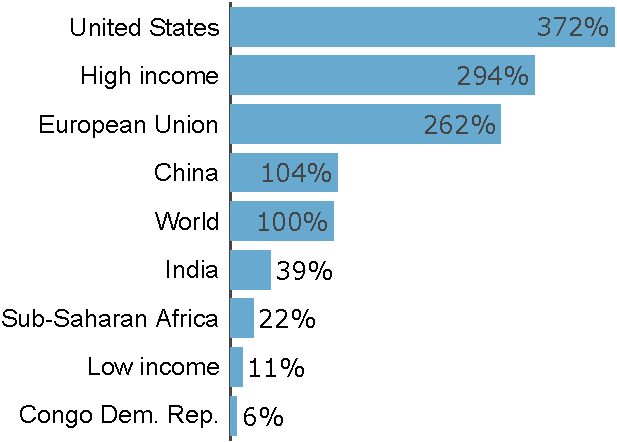
\includegraphics[width=.56\textwidth]{../figures/policies/GDP_pc_PPP_few.pdf}} % https://data.worldbank.org/indicator/NY.GDP.PCAP.PP.CD?contextual=default&end=2021&locations=EU-ZG-XD-XM-1W-IN-US-CD-BI-LU-CN&start=2021&view=bar
\end{figure}

\chapter{La nécessité de redistribution mondiale\label{ch:redistribution_necessaire}}

Qu'elle soit religieuse, philosophique ou intuitive, la morale prescrit généralement des transferts des personnes à hauts revenus vers les personnes à bas revenus, et donc des pays à hauts revenus vers les pays à bas revenus. C'est le cas de l'utilitarisme, la théorie éthique de référence utilisée en économie. L'utilitarisme attribue le même poids à chaque personne et considère ainsi le transfert d'un euro d'une personne riche à une personne pauvre, puisqu'un euro procurera plus de satisfaction à cette dernière. D'après la théorie de la taxation optimale, ce raisonnement est valable tant qu'une augmentation des prélèvements n'incite pas les plus riches à réduire, expatrier ou dissimuler leur activité au point de diminuer les recettes obtenues. En tenant compte de ces effets, des économistes ont calculé qu'un système fiscal optimal reduirait drastiquement les inégalités entre pays et procurerait un revenu minimum de 250\$ par mois au niveau mondial\footnote{Dans ces calculs, \citet{kopczuk_limitations_2005} se limitent à un taux unique (une \textit{flat tax}) et ne s'autorisent pas un barème progressif. Sans cette restriction, le véritable optimum serait encore plus redistributif.}. Pour rationaliser la faiblesse des transferts internationaux, la théorie de la taxation optimale nécessite d'attribuer un poids 2~000 fois plus élevé à un Américain qu'à un Congolais (ou bien, d'attribuer une valeur 100 fois supérieure à l'Américain et de considérer que seul un vingtième de l'argent transféré arrivera à son destinataire, le reste étant détourné par la corruption). %de distordre les poids de sorte que la satisfaction d'un Américain vaille autant que celle de 2~000 Malgaches. 

Au-delà des considérations éthiques, la redistribution mondiale a des fondements juridiques. En 2015, l'ensemble des pays a adopté les Objectifs de développement durable (ODD), au premier rang duquel se trouve l'élimination de l'extrême pauvreté d'ici à 2030. Or, les pays à bas revenus n'ont pas les ressources domestiques suffisantes pour éliminer l'extrême pauvreté. En effet,  dans les 19 pays les plus pauvres, exproprier tous les revenus à partir de 13\$ par jour ne suffirait pas à financer des transferts suffisants pour faire passer leurs 700 millions d'habitants au-dessus de 2\$ par jour d'ici à 2030. Même en faisant l'hypothèse très optimiste d'une croissance du revenu moyen de 7\% par an d'ici à 2030% (soit le maximum observé dans le monde dans les cinq années qui ont précédé la Covid)
, exproprier tous les revenus au-delà de 7\$ par jour ne suffirait pas à éliminer l'extrême pauvreté dans un pays tel que Madagascar\footnote{Ces calculs sont inspirés de \citet{bolch_arithmetics_2022}, reposent sur les données \textit{Poverty and Inequality Platform} de la Banque mondiale, et sont reproductibles sur \href{https://github.com/bixiou/domestic\_poverty\_eradication/code\_poverty/main.R}{github.com/bixiou/domestic\_poverty\_eradication}.}. En d'autres termes, il est impossible d'atteindre le premier ODD sans transferts internationaux. Et ce, alors que le premier ODD se borne à assurer un revenu juste suffisant pour ne plus avoir faim. Le transfert nécessaire correspond à 0,1\% du PIB mondial, soit autant que les dépenses de nourriture pour les animaux de compagnie. % 2019 poverty gap = 2.6% of $2.15 / world GDP of 16865 https://data.worldbank.org/indicator/SI.POV.GAPS; https://www.grandviewresearch.com/industry-analysis/pet-food-industry

Pour s'assurer une vie décente, qui garantit l'accès à l'eau, l'assainissement, l'éducation, à un système de santé, à une certaine mobilité et socialisation, on estime qu'il faut un revenu d'au moins 7\$ par jour\footnote{Cf. \citet{kikstra_decent_2021}}. Près de la moitié des humains vit sous ce seuil de pauvreté\footnote{Cf. \href{https://ourworldindata.org/grapher/distribution-of-population-between-different-poverty-thresholds-up-to-30-dollars}{ourworldindata.org}.}. Combler l'écart qui les sépare de ce seuil coûterait 2 à 3\% du PIB mondial\footnote{En parité de pouvoir d'achat, l'étendue de la pauvreté est de 4 billion de dollar et le PIB mondial de 140 billions.}. % https://data.worldbank.org/indicator/SI.POV.UMIC.GP https://data.worldbank.org/indicator/NY.GDP.MKTP.PP.KD
En outre, 500 millions de personnes vivent dans un pays où le PIB par habitant est inférieur à ce seuil, et où il est donc rigoureusement impossible d'assurer une vie décente à chacun en mobilisant les seules ressources domestiques. 

En 1970, les pays industrialisés ont pris l'engagement d'allouer 0,7\% de leur PIB à l'aide publique au développement, dont 0,2\% du PIB pour les pays les moins avancés. Cet engagement, renouvelé en 2005 et 2015, n'a été jamais été tenu\footnote{Plus exactement, seule une poignée de pays a respecté son engagement : la Suède, la Norvège, le Danemark, le Luxembourg et le Royaume-Uni.}. On estime que l'essentiel des ODD pourraient être atteints si les pays industrialisés respectaient enfin cet engagement\footnote{\citet{sdsn_sdg_2019}}. Pour atteindre une version maximaliste des ODD (y compris assurer l'accès à une énergie propre) ou un autre objectif ambitieux (tel qu'assurer 7\$ par jour à chacun), les pays à hauts revenus devraient transférer davantage de ressources, probablement entre 2 et 6\% de leur PIB. 
% Il va sans dire que pour développer des services de santé, d'éducation, une énergie décarbonée, et plus généralement atteindre l'ensemble des ODD, la solidarité internationale est indispensable. Pour assurer 
% Plus généralement, 12 ODD sur les 17 concernent la pauvreté, les inégalités et le changement climatique. Si les pays à bas revenus n'ont déjà pas les ressources nécessaires pour éliminer l'extrême pauvreté (estimées à 0,1\% du PIB mondial), % 2019 poverty gap = 2.6% of $2.15 / world GDP of 16865 https://data.worldbank.org/indicator/SI.POV.GAPS
% il va sans dire qu'une redistribution internationale est nécessaire pour développer des services de santé, d'éducation, une énergie décarbonée, et plus généralement atteindre l'ensemble des ODD.

De tels transferts seraient colossaux. Mais ils pourraient être intégralement supportés par les millionnaires. En se limitant au millième d'humains les plus riches, qui ont une fortune supérieure à 5 millions d'euros, et en ne taxant que leur fortune au-delà de ce seuil, avec un taux effectif progressant de 1\% pour une fortune de 10 millions d'euros à 10\% pour une fortune de 100 milliards, on récolterait environ 2\% du PIB mondial, et leur fortune ne baisserait même pas (puisque la plupart des milliardaires ont des rendements supérieurs à 10\%). Avec une taxation plus progressive, qui démarrerait à 500~000 euros, avec un taux de 0,25\% pour une fortune d'un million d'euro (soit une taxe de 2~500\euro{} par an), et progresserait jusqu'à un taux de 20\% sur les plus grosses fortunes, les recettes pourraient atteindre 6\% du PIB mondial. Si une telle redistribution était mise en place, les classes moyennes seraient largement épargnées. Certes, des emplois seraient détruits dans le secteur du luxe, puisque les plus fortunés consommeraient un peu moins, mais d'autres secteurs seraient portés par le développement des pays du Sud et créeraient des emplois orientés vers la production de biens exportés, notamment dans l'industrie. 

% TODO? Comment distribuer ? Créer système de protection sociale, cf. ILO Kenya.
% Si les pays de l'OCDE tenaient leur promesse d'allouer 0,7\% de leur PIB à l'aide publique au développement, dont 0,2\% du PIB pour les pays les moins avancés, les ODD pourraient être remplis\footnote{Cf. \citet{sdsn_sdg_2019}.}. 
% Flux dans l'autre sens

Enfin, les transferts internationaux sont une condition sine qua none pour que les pays à bas revenus se décarbonent. D'une part, ces pays font face à d'autres priorités et déploient donc le système énergétique le plus abordable --- reposant souvent sur le charbon. D'autre part, ces pays font valoir --- à juste titre --- qu'ils sont les plus vulnérables au changement climatique alors qu'ils n'y ont contribué que marginalement\footnote{L'Afrique et l'Asie du Sud sont responsables de 6\% des émissions de CO$_\text{2}$ cumulées. % https://ourworldindata.org/contributed-most-global-co2
}. Dans les négociations internationales, ces pays annoncent généralement deux objectifs de réductions d'émissions : un objectif inconditionnel peu ambitieux et un objectif ambitieux conditionnel à des financements extérieurs. Par exemple, l'Éthiopie s'est engagé à réduire inconditionnellement ses émissions de 14\% en 2030 par rapport à un scénario sans action climatique, et conditionne une réduction de 69\% à un financement de 250 milliards de dollar. % https://www.climatewatchdata.org/custom-compare/overview?section=fairness_and_ambition&targets=NGA-revised_first_ndc%2CETH-revised_first_ndc%2CIDN-

Dans les prochains chapitres, nous proposons un Plan mondial pour mettre fin au changement climatique et à l'extrême pauvreté, impliquant d'importants transferts Nord-Sud, tout en étant acceptable pour la population des pays du Nord.
% ODA for LDCs: only Luxembourg is above the objective of 0.2% of GNI (SDG 17.2) https://data.worldbank.org/indicator/DC.ODA.TLDC.GN.ZS?locations=US-GR-LU-SE-GB&most_recent_value_desc=true
% 19 pays (570M en 2022, 700M en 2030) ne pourraient pas éradiquer l'extrême pauvreté même en expropriant tous les revenus au-delà de 13$/jour. Pays comme la RDC ne pourrait pas mettre fin à l'extrême pauvreté en 2030, même avec une croissance de 6% et en expropriant tous les revenus au-delà de 7$/jour.

% Addressing global poverty, inequalities and climate change are at the heart of the universally agreed Sustainable Development Goals (SDG). % 12 out of  17
% It has been pointed out that low-income countries generally do not have enough domestic resources to eliminate the poverty gap in the short run.\cite{bolch_arithmetics_2022} % In other words, it would hardly be possible to achieve the first SDG and end extreme poverty by 2030 without international transfers. => Careful, Bolch use a poverty line above the SDG one.



\chapter{Les grands principes du Plan mondial pour le climat\label{ch:principes}}
% Le plan mondial pour le climat : les grands principes (description de la mesure, des trajectoires)

La proposition développée dans les prochains chapitres ne résout pas tous les problèmes de l'humanité, et ne constitue pas non plus une réponse complète au changement climatique. Si elle est désignée <<~Plan mondial pour le climat~>> parce que ça sonne bien, <<~Cadre international de sortie des énergies fossiles~>> aurait été plus fidèle.  % Une désignation telle que <<~Cadre international de sortie des énergies fossiles~>> aurait été plus fidèle, mais il faut dire que <<~Plan mondial pour le climat~>> sonne mieux. %C'est donc peut-être exagéré de le nommer <<~Plan mondial pour le climat~>>, mais ça sonne mieux qu'une désignation plus fidèle telle que <<~Cadre international de sortie des énergies fossiles~>>. 
En effet, ce plan couvre uniquement les émissions de CO$_\text{2}$ fossiles et industrielles, pas celles liées à l'usage des terres, à la forêt ou aux autres gaz à effet de serre. Sa portée se limite à établir un cadre qui garantit les réductions d'émissions et détermine les transferts internationaux, sous la forme d'un traité. Charge ensuite à chaque État ou collectivité de prendre les mesures (climatiques ou sociales) appropriées pour que la décarbonation se passe bien sur son territoire. 

\section{Le cœur du Plan}

On a vu au chapitre \ref{ch:statu_quo} que l'humanité disposait d'un budget carbone à ne pas dépasser pour maintenir le réchauffement sous une cible donnée. L'accord de Paris fournit cette cible. En effet, l'intégralité des pays a signé cet accord en 2015, et visent ainsi à contenir le réchauffement <<~nettement en dessous de 2\textdegree{}C (...) en poursuivant l'action menée pour limiter l'élévation de température à 1,5\textdegree{}C~>>. 

Comment garantir une trajectoire d'émissions conforme à ce budget carbone~? Le plus sûr serait de plafonner les émissions mondiales, avec un plafond annuel qui décroît en conformité avec l'objectif. 

Comment alors allouer les permis d'émissions de CO$_\text{2}$~? Le plus naturel % simple, élémentaire
est d'allouer un même permis d'émission à chaque humain. 

Faut-il autoriser la revente des permis d'émissions~? Oui. % Passer en FAQ la suite ?
Instaurer un marché du carbone est préférable à un système de quota carbone non échangeable pour plusieurs raisons. Déjà, si les permis d'émissions ne sont pas échangeables, cela signifie soit que des centaines millions de personnes (notamment dans les pays du Nord) devraient diviser leurs émissions par deux ou trois du jour au lendemain (les mettant dans l'impossibilité de poursuivre leurs activités), soit qu'on allouerait (dans un premier temps) davantage de permis d'émissions aux personnes qui polluent davantage (ce qui romprait avec le principe d'égalité cher aux défenseurs des quotas non échangeables). A contrario, si les permis sont échangeables, les pollueurs auraient une certaine latitude pour choisir leurs émissions et du temps pour adapter progressivement leurs activités et changer leur équipement, tandis que les personnes avec une faible empreinte carbone pourraient revendre leurs permis d'émissions inutilisés et ainsi gagner du pouvoir d'achat. Ainsi, tant les pollueurs que les frugaux bénéficieraient de la flexibilité permise par le marché. D'ailleurs, le bénéfice potentiel serait tellement important que l'émergence d'un marché noir serait difficile à empêcher dans le cas d'un système de quotas non échangeables. Vous vous dites peut-être qu'un marché du carbone serait immoral ou injuste, car il permettrait aux plus riches de continuer à polluer. Pourtant, un tel système opérerait une redistribution des pollueurs vers les frugaux : ceux-là devant payer pour acheter des permis d'émissions à ceux-ci. En outre, mettre en place un marché du carbone n'empêche pas d'interdire par ailleurs les consommations jugées superflues, telles que les yachts, les jets privés, voire les SUV. Enfin, si on considère injuste que les plus riches soient capables de préserver un mode de vie dispendieux dans un tel système, n'est-ce pas parce qu'on considère l'extrême richesse comme injuste ? Si c'est le cas, autant s'attaquer à la fortune directement, plutôt que de passer par des moyens détournés. En effet, plafonner les émissions de Rupert Murdoch ne l'empêcherait pas d'utiliser son empire médiatique pour minimiser, voire nier le changement climatique. %d'Elon Musk ne l'empêcherait pas d'acheter Twitter et d'en contrôler l'algorithme. 

% Un dernier argument contre le marché est qu'il permettrait des enrichissements illégitimes à cause de la fraude ou la spéculation. 

Pour l'instant, j'ai fait comme si les individus auraient la responsabilité d'acheter ou vendre des permis d'émissions, alors qu'on ne sait même pas mesurer précisément les émissions de quelqu'un. En réalité, on peut obtenir des effets équivalents au système décrit précédemment avec un fonctionnement bien plus simple. 

Chaque année, un nombre limité de permis d'émissions serait créé, en conformité avec la trajectoire d'émissions qu'on s'est fixée. Ces permis d'émissions seraient mis aux enchères auprès des entreprises à la source des émissions de CO$_\text{2}$, et en particulier celles qui extraient du charbon, du pétrole ou du gaz. Ces entreprises devraient se procurer des permis correspondant à leurs émissions. Enfin, les recettes générées par la vente de permis seraient redistribuées en un revenu de base égal pour tous les humains. 

D'un point de vue théorique, ce système est équivalent au précédent. En effet, les entreprises polluantes répercuteront le coût des permis d'émissions en hausse de prix, de sorte que les consommateurs feront face à une hausse de prix égal au prix du carbone multiplié par leur empreinte carbone. Quant aux recettes générées, elles correspondront au produit de l'empreinte carbone par l'ensemble des émissions, de sorte que le revenu de base serait égal au prix du carbone multiplié par l'empreinte carbone moyenne. Dans le système précédent, les permis d'émissions sont alloués de façon égalitaire aux individus, donc les permis d'émissions d'un individu correspondent à l'empreinte carbone moyenne. Ainsi, si une personne revend tous ses permis d'émissions, elle toucherait un montant équivalent au revenu de base. Par ailleurs, cette personne devrait alors acheter des permis pour couvrir ses émissions, pour un montant égal au prix du carbone multiplié par son empreinte. Dans les deux cas, on retombe sur le même calcul. Le système individuel est intéressant d'un point de vue théorique, puisqu'il permet de montrer l'équivalence entre allocation des permis d'émissions et allocation des recettes d'une tarification carbone. En revanche, le système d'enchères aux entreprises est le seul qui soit réaliste à administrer. 

Pour résumer, on peut mettre fin au réchauffement climatique en plafonnant les émissions et éliminer l'extrême pauvreté à l'aide d'un revenu de base. Un système simple et efficace pour traiter ces deux problèmes est de combiner ces deux solutions. Voici le cœur du Plan mondial pour le climat, qui constituent les deux premiers principes détaillés ci-dessous. Pour des considérations de justice et de géopolitique, quelques ajustements sont nécessaires pour compléter notre proposition : je les décris ci-après aux principes 3 et 4. Enfin, ce Plan mondial pour le climat doit être complémenté par d'autres mesures : je les esquisse au chapitre \ref{ch:premier_pas}.

\section{1$^\text{er}$ principe~: Un quota annuel d'émissions}

Le budget carbone --- et avec lui le climat futur --- est l'élément décisif que les États devront négocier. Dans ce livre, nous interprétons l'accord de Paris comme permettant un dépassement temporaire de la cible de 1,5\textdegree{}C dès lors que le réchauffement n'excède pas 2\textdegree{}C. En d'autres termes, des émissions négatives nettes (à partir de la deuxième moitié de ce siècle) permettront de redescendre jusqu'à 1,5\textdegree{}C, seuil qui sera très probablement déjà franchi en 2040\footnote{\citet{diffenbaugh_data-driven_2023} estiment que le réchauffement dépassera 1,5\textdegree{}C en 2035 dans un scénario de décarbonation ambitieuse, ce qui est cohérent avec la Table 4.2 du rapport de l'\citet{ipcc_climate_2021}}. 

Notre proposition repose sur deux budgets carbone~: un budget d'émissions positives, conforme à l'objectif de ne pas dépasser les 2\textdegree{}C de réchauffement, et un budget d'émissions négatives, permettant de réduire la température. Pour fixer les idées, disons que le budget d'émissions positives serait de 1~000 GtCO$_\text{2}$ à partir de 2025, et le budget d'émissions négatives serait de 500 GtCO$_\text{2}$, ce qui signifie que le budget d'émissions nettes serait de $1~000-500=500$ GtCO$_\text{2}$. Pour l'instant, ne nous préoccupons pas des émissions négatives, qui ne prendront leur essor quand dans quelques décennies. 
% Faire différemment pour gérer le plastique : budget carbone jusqu'à net zéro, puis double budget (positif et négatif)
% Pb du plastique: si on le fait payer à l'extraction, on a intérêt à extraire, stocker sous forme de plastiques, et brûler plus tard quand la tonne est plus chère. Comment faire ?

L'organe décisionnaire du Plan définirait le quota annuel d'émissions (positives), selon une trajectoire conforme au budget carbone. En début d'année, ce quota serait mis aux enchères sous la forme de permis d'émissions d'une tonne de CO$_\text{2}$. Les sociétés assujetties seraient les entreprises ``upstream'', c'est-à-dire celles qui extraient des hydrocarbures, importent des biens depuis des pays non participants, ou produisent du ciment. Chaque société assujettie transmettrait une liste de quantité de permis qu'elle s'engage à acheter pour différents niveaux de prix. Pour chaque niveau de prix, on obtient ainsi une quantité agrégée demandée par les sociétés assujetties. Les permis sont alors vendus au prix pour lequel la quantité demandée correspond au quota. Les sociétés assujetties et des sociétés financières agréées peuvent ensuite échanger des permis d'émissions sur un marché secondaire. Au bout de quelques années (probablement un ou deux), le prix d'équilibre aura été découvert, de sorte que le prix sur le marché secondaire sera relativement stable et égal à celui des enchères. En fin d'année, les émissions issues des entreprises assujetties seraient contrôlées, et elles devraient délivrer des permis correspondant à ces émissions. Des sanctions dissuasives garantiraient le bon fonctionnement du système. Par exemple, pour toute tonne de CO$_\text{2}$ non couverte par un permis d'émissions, la société assujettie devrait payer une amende égale à trois fois le prix d'une tonne de CO$_\text{2}$, et devrait délivrer le permis manquant l'année suivante. 

En résumé, un système d'échange de permis d'émission (ETS, pour \textit{emissions trading system}) serait mis en place pour plafonner les émissions de CO$_\text{2}$ au niveau mondial. 
Un tel système a déjà fait ses preuves dans plusieurs pays, dont l'Union Européenne\footnote{L'ETS européen est souvent décrié. Pourtant, il y a bel et bien permis de réduire les émissions couvertes (celles de l'industrie et de la production d'électricité) conformément à l'objectif fixé, tandis que les émissions non couvertes (mais qui vont l'être à partir de 2027) ont continué de croître. En réalité, l'ETS européen a été critiqué pour deux (bonnes) raisons. D'une part, l'objectif fixé n'était pas assez ambitieux (c'est ce qui explique le prix très faible jusqu'à une réforme du système en 2019). D'autre part, les permis d'émissions étaient attribués gratuitement aux entreprises polluantes, plutôt que vendus aux enchères. Ces deux écueils seront évités dans le Plan mondial pour le climat.}, la Chine et la Corée du Sud, et est à l'étude dans d'autres comme l'Inde, le Brésil ou le Nigeria. 17\% des émissions mondiales sont déjà couvertes par un ETS. Différents peuvent être fusionnés avec succès, comme l'ont montré la Californie et le Québec\citep{icap_emissions_2023}. 
% Plan en +, pas fusion
% Détails on sait faire, pas besoin d'en parler ici

\section{2$^\text{e}$ principe~: Un revenu de base mondial}

\section{3$^\text{e}$ principe~: Un club climatique}

\section{4$^\text{e}$ principe~: Des mécanismes de participation}

% 1.	Plafonner les émissions en conformité avec une trajectoire +2°C, à l’aide d’un ETS
% •	Le traité définirait un budget carbone, ensuite décliné en quotas annuels.
% •	Des permis d’émissions de CO2 seraient vendus aux enchères aux entreprises émettrices, comme dans le marché du carbone (ETS) européen.	
% •	Le prix du carbone inciterait les ménages et entreprises à se décarboner. 
% •	Il serait in fine payé par les individus en proportion de leur empreinte carbone.	

% 2.	Utiliser les recettes pour verser un revenu de base mondial et résorber la pauvreté
% •	Les recettes seraient reversées sous la forme d’un revenu de base à tous les adultes.
% •	Chaque humain recevrait ainsi environ 50€/mois.
% •	Les versements sont techniquement possibles (smartphones, internet par satellites).

% 3.	Former un club climatique avec une tarification carbone aux frontières
% •	Le traité entrerait en vigueur dès que les entités signataires couvrent 60% des émissions mondiales (Chine : 30%, pays bénéficiaires nets : 23%, UE+UK : 9%, U.S. : 15%).
% •	Les importations vers le club seraient taxées en proportion de leur contenu carbone.

% 4.	Inclure des mécanismes qui encouragent la participation de la Chine, la Californie… 
% •	Le traité permettrait à des États de rejoindre l’accord indépendamment du niveau fédéral, notamment en les exemptant de la tarification aux frontières.
% •	Une clause d’opt out de la mutualisation des recettes permettrait à des pays (comme la Chine, l’Afrique du Sud ou l’Algérie) dont le PIB par habitant n’excède pas la moyenne mondiale de plus de 50% de conserver les recettes prélevées sur leur territoire, leur évitant d’être contributeur net malgré leur empreinte carbone supérieure à la moyenne.

% 5.	Complémenter ce Plan par d’autres mesures pour le climat et la justice sociale
% •	Une fiscalité plus progressive pour compenser les classes moyennes des pays riches.
% •	Un ISF mondial finançant les pays pauvres pour traiter les responsabilités historiques.
% •	Des mesures climatiques nationales pour faciliter la décarbonation.


\chapter{Les détails du Plan\label{ch:details}}
% Le plan mondial pour le climat : les détails (implémentation, mécanismes de participation)

\chapter{Un transfert massif vers les pays du Sud\label{ch:effets_distributifs}}
% Le plan mondial pour le climat : les effets distributifs (carte des pays gagnants et perdants)

% Une redistribution de 1% de PIB mondial des pays riches vers les pays pauvres.
% •	Le Plan opérerait une redistribution des individus avec une empreinte carbone élevée vers ceux avec une empreinte faible. L’effet serait nul au niveau de la moyenne mondiale.
% •	Lors de leur plateau, entre 2030 et 2050, les recettes correspondraient à environ 5% du PIB mondial, dont 1% en transferts nets entre pays.
% •	Le Français moyen perdrait 14€/mois au pic, soit une perte de 0,4% du revenu national.
% •	Le revenu de base sortirait de l’extrême pauvreté les 700 millions vivant sous les 2$/jour.
% •	Ces estimations ont été faites avec le scénario +2°C central du GIEC, qui implique un prix du carbone d’environ 150$/tCO2 en 2030, 200$ en 2040, 400$ en 2050, et net zéro en 2070.


\chapter{Un Plan largement soutenu\label{ch:soutien}}

% Un plan largement soutenu (soutien majoritaire dans 20 pays, avantage électoral aux partis de gauche qui l'incluraient dans leur programme, consensus en faveur de la répartition égalitaire de l'effort de décarbonation)

\chapter{Un pas vers un monde soutenable\label{ch:premier_pas}}
% Un pas vers un monde soutenable (le Plan n'est pas suffisant, il doit être complémenté d'autres mesures climatiques (nationales, sectorielles), d'autres mesures de redistribution mondiale (impôt sur la fortune), et l'objectif de long terme doit être d'assurer les conditions nécessaires au bien-être à chaque humain)

\chapter{L'appel pour la redistribution mondiale\label{ch:appel}}
% L'appel pour la redistribution mondiale (description de l'activité de Global Redistribution Advocates, lien vers la lettre ouverte aux dirigeants pour la redistribution mondiale - que nous prévoyons de publier dans les grands journaux type The Guardian, Le Monde..., appel à une manifestation mondiale en soutien à cet appel le 1er décembre 2024 lors de la COP29).

\chapter{Foire Aux Questions\label{ch:faq}}


% \begin{center}
% {\textbf{\href{https://github.com/bixiou/global_tax_attitudes/raw/main/paper/book.pdf}{Link to most recent version}}}
% \end{center}

% 0. Préface : j'envisage Thomas Piketty, Jean Tirole, Gaël Giraud ou Esther Duflo pour la version française et Greta Thunberg ou Joseph Stiglitz pour la version anglaise (mais ça reste à définir)
% 1. Un statu quo insupportable : l'extrême pauvreté, le changement climatique (chiffres, constat)
% 2. La nécessité de redistribution mondiale (objectifs de développement durable, justifications théoriques)
% 3. Le plan mondial pour le climat : les grands principes (description de la mesure, des trajectoires)
% 4. Le plan mondial pour le climat : les détails (implémentation, mécanismes de participation)
% 5. Le plan mondial pour le climat : les effets distributifs (carte des pays gagnants et perdants)
% 6. Un plan largement soutenu (soutien majoritaire dans 20 pays, avantage électoral aux partis de gauche qui l'incluraient dans leur programme, consensus en faveur de la répartition égalitaire de l'effort de décarbonation)
% 7. Un pas vers un monde soutenable (le Plan n'est pas suffisant, il doit être complémenté d'autres mesures climatiques (nationales, sectorielles), d'autres mesures de redistribution mondiale (impôt sur la fortune), et l'objectif de long terme doit être d'assurer les conditions nécessaires au bien-être à chaque humain)
% 8. L'appel pour la redistribution mondiale (description de l'activité de Global Redistribution Advocates, lien vers la lettre ouverte aux dirigeants pour la redistribution mondiale - que nous prévoyons de publier dans les grands journaux type The Guardian, Le Monde..., appel à une manifestation mondiale en soutien à cet appel le 1er décembre 2024 lors de la COP29).
% 9. Postface : Foire Aux Questions (description et réponse aux objections habituelles)

% Un plan mondial pour le climat et contre l'extrême pauvreté (version courte illustrée / version longue) :
% - situation pauvreté, csq CC
% - SDGs, justifications redistr. mondiale
% - description GCS, y.c. trajectoires
% - détails implémentation (e.g. Aadhaar)
% - acceptation
% - autres mesures mondiales possibles
% - appel signé par milliers + manif mondiale un an après lancement
% - préface Piketty puis Greta
% - FAQ, y.c. critiques d'une page (et réponses) de Piketty, etc.
% Opuscule Cepremap au pire

% FAQ
% - Les émissions vont augmenter si on distribue un revenu de base et les revenus augmentent
% - Qui paient : entreprises ou consommateurs ?
% - Les quotas profitent aux plus riches qui peuvent s'acheter plus de quotas, les plus pauvres bradent leurs quotas pour des rétributions immédiates en obérant des potentialités pour le futur 
% - pas sûr que ça ait fait ses preuves 
% - il y a certaines pratiques qui vont devoir s'arrêter, il faut interdire
% => Le Plan fournit un cadre qui assure des réductions d'émissions adéquates; qui incite les États à prendre des mesures complémentaires type interdiction; on peut remplacer le système d'échanges de permis par une taxe, c'est équivalent. 
% Pourquoi pas taxe progressive ?
% Problème de la fraude / du monitoring.
% Problème de la transparence sur les implications (les gens réalisent-ils les changements de mode de vie nécessaires ?)
% Qu'est-ce qu'on fait de l'EU ETS? On le laisse en place. 
% Les taxes affectées ne sont-elles pas interdites ? => no, e.g. Chirac tax on flying

% Wealth tax: 
% taxe universelle ? exit tax ?

\renewcommand{\url}[1]{\href{#1}{Link}} % NCCcomment
\bibliographystyle{plainnaturl_clean} % NCCcomment
\bibliography{global_tax_attitudes}

\end{document}